\documentclass{article}
% ~ ~ ~ ~ ~ ~ ~ ~ ~ ~ ~ ~ ~ ~ ~ ~ ~ ~ ~ ~ ~ ~ ~ ~ ~ ~ ~ ~ ~ ~ ~ ~ ~ ~ ~ ~ ~ ~ ~ ~ ~ ~ ~ ~ ~ ~ ~ ~

\usepackage[utf8]{inputenc}
\usepackage{amsmath}
\usepackage{amssymb} % for \mathbb
\usepackage{graphicx} % for figures
\usepackage{color}
\usepackage[usenames,dvipsnames]{xcolor}
\usepackage{hyperref} % for hyperlinks
\usepackage{float} % for figures
% ~ ~ ~ ~ ~ ~ ~ ~ ~ ~ ~ ~ ~ ~ ~ ~ ~ ~ ~ ~ ~ ~ ~ ~ ~ ~ ~ ~ ~ ~ ~ ~ ~ ~ ~ ~ ~ ~ ~ ~ ~ ~ ~ ~ ~ ~ ~ ~
% CUSTOM COLOUR
\definecolor{DGrey}{rgb}{0.1,0.1,0.1} % Dark Grey
% ~ ~ ~ ~ ~ ~ ~ ~ ~ ~ ~ ~ ~ ~ ~ ~ ~ ~ ~ ~ ~ ~ ~ ~ ~ ~ ~ ~ ~ ~ ~ ~ ~ ~ ~ ~ ~ ~ ~ ~ ~ ~ ~ ~ ~ ~ ~ ~
\title{ Introduction to Engineering Written Assignment Questions}
\date{January 2013}
\author{Greg Mayer and Daniel Connelly}
% ~ ~ ~ ~ ~ ~ ~ ~ ~ ~ ~ ~ ~ ~ ~ ~ ~ ~ ~ ~ ~ ~ ~ ~ ~ ~ ~ ~ ~ ~ ~ ~ ~ ~ ~ ~ ~ ~ ~ ~ ~ ~ ~ ~ ~ ~ ~ ~
% HEADER/FOOTER
\usepackage{fancyheadings}
\pagestyle{myheadings} % set headings to be user defined
\fancyhead{} % To create custom header, clear default layout
\renewcommand{\subsectionmark}[1]{\markright{{\color{DGrey}\thesubsection} \ {\color{DGrey}#1}}}
\fancyhead[LE,LO]{\subsectionmark} % To create custom header, clear default layout

% ~ ~ ~ ~ ~ ~ ~ ~ ~ ~ ~ ~ ~ ~ ~ ~ ~ ~ ~ ~ ~ ~ ~ ~ ~ ~ ~ ~ ~ ~ ~ ~ ~ ~ ~ ~ ~ ~ ~ ~ ~ ~ ~ ~ ~ ~ ~ ~
% ENUMERATION

\usepackage{enumitem}   % so that question numbers can be formatted 
\setenumerate[1]{label=\thesubsection.\arabic*.} % enumerate environment: add section numbers to items
% ~ ~ ~ ~ ~ ~ ~ ~ ~ ~ ~ ~ ~ ~ ~ ~ ~ ~ ~ ~ ~ ~ ~ ~ ~ ~ ~ ~ ~ ~ ~ ~ ~ ~ ~ ~ ~ ~ ~ ~ ~ ~ ~ ~ ~ ~ ~ ~
% MARGINS
\usepackage{anysize}
\marginsize{2.5cm}{2.5cm}{1cm}{1cm}
% ~ ~ ~ ~ ~ ~ ~ ~ ~ ~ ~ ~ ~ ~ ~ ~ ~ ~ ~ ~ ~ ~ ~ ~ ~ ~ ~ ~ ~ ~ ~ ~ ~ ~ ~ ~ ~ ~ ~ ~ ~ ~ ~ ~ ~ ~ ~ ~
% PAGE NUMBERING
\pagenumbering{arabic}
% ~ ~ ~ ~ ~ ~ ~ ~ ~ ~ ~ ~ ~ ~ ~ ~ ~ ~ ~ ~ ~ ~ ~ ~ ~ ~ ~ ~ ~ ~ ~ ~ ~ ~ ~ ~ ~ ~ ~ ~ ~ ~ ~ ~ ~ ~ ~ ~
% Custom Commands
\newcommand{\Emph}[1]{\textbf{#1}} % Emphasize
\newcommand{\R}{\mathbb{R}} 
\newcommand{\BM}{\begin{bmatrix}} % Begin Matrix
\newcommand{\EM}{\end{bmatrix}} % End Matrix
\newcommand{\BEN}{\begin{enumerate}[leftmargin=1.1cm]}% Begin ENumerate
\newcommand{\EEN}{\end{enumerate}} % End ENumerate
\newcommand{\MB}{\mathbf} % Math Bold

\newcommand{\px}{\frac{\partial}{\partial x}} % Partial wrt x
\newcommand{\py}{\frac{\partial}{\partial y}} % Partial wrt y

\newcommand{\pfx}{\frac{\partial f}{\partial x}} % Partial of f wrt x
\newcommand{\pfy}{\frac{\partial f}{\partial y}} % Partial of f wrt y
\newcommand{\pfxy}{\frac{\partial^2 f}{\partial y \partial x}} % Partial of f wrt y
\newcommand{\pfyx}{\frac{\partial^2 f}{\partial x \partial y}} % Partial of f wrt y

\newcommand{\ux}{\frac{\partial u}{\partial x }} % Partial of u wrt x
\newcommand{\uk}{\frac{\partial u}{\partial k }} % Partial of u wrt k
\newcommand{\ut}{\frac{\partial u}{\partial t}} % Partial of u wrt t
\newcommand{\utt}{\frac{\partial^2u}{\partial t^2}} % Partial of u wrt t
\newcommand{\us}{\frac{\partial u}{\partial s}} % Partial of u wrt t
\newcommand{\uss}{\frac{\partial^2 u}{\partial s^2}} % Partial of u wrt t
\newcommand{\kx}{\frac{\partial k}{\partial x }} % Partial of k wrt x
\newcommand{\kt}{\frac{\partial k}{\partial t }} % Partial of k wrt t

\newcommand{\pxu}{\frac{\partial x}{\partial u}} % x wrt u
\newcommand{\pxv}{\frac{\partial x}{\partial v}} % x wrt v
\newcommand{\pxw}{\frac{\partial x}{\partial w}} % x wrt v
\newcommand{\pxt}{\frac{\partial x}{\partial t}} % x wrt t
\newcommand{\pyu}{\frac{\partial y}{\partial u}} % y wrt u
\newcommand{\pyv}{\frac{\partial y}{\partial v}} % y wrt v
\newcommand{\pyw}{\frac{\partial y}{\partial w}} % y wrt v
\newcommand{\pyt}{\frac{\partial y}{\partial t}} % y wrt t
\newcommand{\pzu}{\frac{\partial z}{\partial u}} % z wrt u
\newcommand{\pzv}{\frac{\partial z}{\partial v}} % z wrt v
\newcommand{\pzw}{\frac{\partial z}{\partial w}} % z wrt v
\newcommand{\pzt}{\frac{\partial z}{\partial t}} % z wrt t


\newcommand{\VCT}{\textit{Vector Calculus} by Michael Corral} % Vector Calculus Textbook
\newcommand{\CAT}{\textit{College Algebra} by Carl Stitz and Jeff Zeager} % College Algebra Textbook
\newcommand{\From}{The following questions are related to } % Questions ....
% ~ ~ ~ ~ ~ ~ ~ ~ ~ ~ ~ ~ ~ ~ ~ ~ ~ ~ ~ ~ ~ ~ ~ ~ ~ ~ ~ ~ ~ ~ ~ ~ ~ ~ ~ ~ ~ ~ ~ ~ ~ ~ ~ ~ ~ ~ ~ ~
% ONLY USED FOR EDITING
\newcommand{\rednote}[1]{{\color{red}\textit{\textbf{#1}}}} % Shortcut for formatting notes for developers
\newcommand{\FromC}[1]{{\color{DGrey}\textit{#1}}} % Shortcut for coloring the "from" text
% ~ ~ ~ ~ ~ ~ ~ ~ ~ ~ ~ ~ ~ ~ ~ ~ ~ ~ ~ ~ ~ ~ ~ ~ ~ ~ ~ ~ ~ ~ ~ ~ ~ ~ ~ ~ ~ ~ ~ ~ ~ ~ ~ ~ ~ ~ ~ ~
% AUGMENTED MATRIX MACRO
% thanks to http://tex.stackexchange.com/questions/2233/whats-the-best-way-make-an-augmented-coefficient-matrix
\newenvironment{amatrix}[1]{%
  \left[\begin{array}{@{}*{#1}{c}|c@{}}
}{%
  \end{array}\right]
}
% ~ ~ ~ ~ ~ ~ ~ ~ ~ ~ ~ ~ ~ ~ ~ ~ ~ ~ ~ ~ ~ ~ ~ ~ ~ ~ ~ ~ ~ ~ ~ ~ ~ ~ ~ ~ ~ ~ ~ ~ ~ ~ ~ ~ ~ ~ ~ ~
% PAGE LAYOUT
\addtolength{\topmargin}{10pt}
\addtolength{\headsep}{10pt}
\addtolength{\textheight}{-20pt}


\usepackage{multienum}
\usepackage{wrapfig}

\date{}
% ~ ~ ~ ~ ~ ~ ~ ~ ~ ~ ~ ~ ~ ~ ~ ~ ~ ~ ~ ~ ~ ~ ~ ~ ~ ~ ~ ~ ~ ~ ~ ~ ~ ~ ~ ~ ~ ~ ~ ~ ~ ~ ~ ~ ~ ~ ~ ~
\begin{document}
\begin{center}
\textsc{\LARGE Written Assignment 2}\\[0.5cm]
\end{center}

\section*{Questions}

\begin{enumerate}
% ~~~~~~~~~~~~~~~~~~~~~~~~~~~~~~~~~~~~~~~~~~~~~~~~~~~~~~~~~
\item 
% QUESTION
% GPS: Not in GPS
For the following functions, 
\begin{itemize}
\item determine the domain of the function,
\item sketch the domain of the function in the $xy$ plane, and
\item determine the range of the function
\end{itemize}
\begin{enumerate}
  \item $f(x,y) = \frac{1}{\sqrt{(x-1)(y-1)}}$
  \item $g(x,y) = \frac{\sqrt{x+1}}{yx^2+xy^2}$
  \item $h(x,y) = \frac{xyz}{x^2+y^2-1}$
  \item $z(x,y) = \ln(x+2y)$
\end{enumerate}
% ~~~~~~~~~~~~~~~~~~~~~~~~~~~~~~~~~~~~~~~~~~~~~~~~~~~~~~~~~
\item 
% QUESTION
%GPS: MMCD1
Evaluate the following limits or show that they do not exist.  
\begin{enumerate}
\item $\displaystyle \lim_{(r,s)\rightarrow(0,2\pi) } \frac{3r^2+rs^3-3r^4\sin (s/4)}{r^2}$
\item $\displaystyle \lim_{(x,y)\rightarrow(0,0) } \frac{x-y}{x+y}$
\item $\displaystyle \lim_{(x,y,z)\rightarrow(1,1,1)} \big|3x - 2y - z \big|$
\item $\displaystyle \lim_{(x,y,z)\rightarrow(0,0,0) } \frac{x^2-y^2-z^2}{x^2+y^2+z^2}$
\item $\displaystyle \lim_{(x,y)\rightarrow(1,0) } \frac{\sqrt{2x+y}-\sqrt{2x-y}}{2y}$
\end{enumerate}
% ~~~~~~~~~~~~~~~~~~~~~~~~~~~~~~~~~~~~~~~~~~~~~~~~~~~~~~~~~
\item 
% QUESTION
%GPS: MMCD1
Consider the function
\begin{align*}
g(x,y,z) = \left\{
\begin{array}{rl}
1 & \text{if } (x,y,z) = (0,0,1) \\
x + y + 2z & \text{if } (x,y,z) \ne (0,0,1) 
\end{array} \right. .
\end{align*}
Find all points or regions where $g(x,y,z)$ has a discontinuity.
% ~~~~~~~~~~~~~~~~~~~~~~~~~~~~~~~~~~~~~~~~~~~~~~~~~~~~~~~~~
\item 
% QUESTION
%GPS: MMCD1
Evaluate the following limit, if it exists.
\begin{align*} 
\lim_{(x,y)\rightarrow(1,0) } \frac{x(x-1)^3 + y^2}{4(x-1)^2+9y^3}
\end{align*}
 \textit{Hint: approach the limit point along straight lines}.
% ~~~~~~~~~~~~~~~~~~~~~~~~~~~~~~~~~~~~~~~~~~~~~~~~~~~~~~~~~
\item 
% QUESTION
%GPS: MMCA3b
Sketch, by hand, the level curves of the following functions for the indicated values of $c$, if possible. You may of course want to check your answer using a calculator or with graphing software. 
\begin{enumerate}
\item $f(x,y) =\frac{\ln y}{x^2} $, $c=-2, - 1, 0 , 1 , 2$
\item $f(x,y) = \frac{x^2}{x^2+y^2}$, $c=0,\frac{1}{4},\frac{1}{2},1,2$
\end{enumerate}
% ~~~~~~~~~~~~~~~~~~~~~~~~~~~~~~~~~~~~~~~~~~~~~~~~~~~~~~~~~
\item 
% QUESTION
%GPS: MMCA3b
\begin{enumerate}
\item Find a function $f(x,y)$ whose family of level curves are straight lines that pass through the point $(2,1)$.
\item Find a function $f(x,y)$ whose family of level curves are circles with radius $\sqrt{e^c}$. 
\end{enumerate}

% ~~~~~~~~~~~~~~~~~~~~~~~~~~~~~~~~~~~~~~~~~~~~~~~~~~~~~~~~~
\item Let $m$ be any real number. 
\begin{enumerate}
\item Provide an example of a function, $f(x,y)$, with the following two properties:
\begin{itemize}
\item $f(x,y) \rightarrow m$ as $(x,y) \rightarrow (1,0)$ along any parabola, $y=m(x-1)^2$
\item $f(x,y)$ is not constant
\end{itemize}
\item Explain why the limit you provided in part (a) does not exist. 
\end{enumerate}
% ~~~~~~~~~~~~~~~~~~~~~~~~~~~~~~~~~~~~~~~~~~~~~~~~~~~~~~~~~
% TEMPERATURE DISTRIBUTION
\item \textbf{Application to Temperature Distributions}\\
Suppose that a metal object occupies a space in three dimensions, and that the temperature, $T(x,y)$ of the object at the point $(x,y)$ is inversely proportional to the distance between the point and the origin. 
\BEN
\item Write down an expression for $T$ as a function of $x$ and $y$.
\item Describe the level curves in words. Sketching them is not necessary, but the level curves are known as \Emph{isothermals}, and represent curves upon which the temperature is constant. 
\item Suppose the temperature of the object at the point (2,1) is $10^{\circ}$C. Find the temperature of the object at (1,3).
\EEN
% ~~~~~~~~~~~~~~~~~~~~~~~~~~~~~~~~~~~~~~~~~~~~~~~~~~~~~~~~~
% ELECTRICAL FIELD DISTRIBUTION
\item \textbf{Application to Electrical Potential Distributions}\\
The scalar function
\begin{align*}
V(x,y) = \frac{c}{\sqrt{r^2 - x^2 -y^2}}\ ,
\end{align*}
where $c$ and $r$ are positive constants, represents the electrical potential (in volts) at a point $(x,y)$ in the $xy-$plane. Describe, in words, the level curves $V(x,y)=K$ for constant $K\in\R$, and determine the values of $K$ for which the curves exist. Note that the level curves are known as \Emph{equipotential curves}, because all points on a given curve have the same potential. \textit{can we do something a little more interesting with this question? its somewhat similar to the previous one}

% ~~~~~~~~~~~~~~~~~~~~~~~~~~~~~~~~~~~~~~~~~~~~~~~~~~~~~~~~~
\item 
% BONUS QUESTION, LIMITS
\textbf{Bonus Problem}\\
\textit{This question goes beyond the requirements for this course. Before starting this problem, make sure that your instructor will give you marks for solving it.} \\
Using the definition of limit (the $\epsilon, \delta$ definition) for a function of two variables, prove that the limit
\begin{align*}
\lim_{(x,y)\rightarrow(0,0) } \frac{xy^2}{x^2+y^2}
\end{align*}
exists. \textit{Hint: start by evaluating the limit along the $x$-axis, or along other straight lines to determine what the limit could be equal to}.
% ~~~~~~~~~~~~~~~~~~~~~~~~~~~~~~~~~~~~~~~~~~~~~~~~~~~~~~~~~
\end{enumerate}
\noindent \textbf{References} \\
The temperature and electrical potential questions are based on a similar exercises that can be found in \textit{Calculus, One and Several Variables}, 10th Edition, by Salas, Hille, Etgen, Wiley, 2007.
%%%%%%%%%%%%%%%%%%%%%%%%%%%%%%%%%%%%%%
%%%%%%%%%%%%%%%%%%%%%%%%%%%%%%%%%%%%%%
%%%%%%%%%%%%%%%%%%%%%%%%%%%%%%%%%%%%%%

% SOLUTIONS
\newpage
\section*{Solutions}
\begin{enumerate}
% ~~~~~~~~~~~~~~~~~~~~~~~~~~~~~~~~~~~~~~~~~~~~~~~~~~~~~~~~~
%DOMAIN AND RANGE PROBLEMS
\item 
\begin{enumerate}
% -  -  -  -  -  -  -  -  -  -  -  -  -  -  -  -  -  -  -  -  -  -  -  -  -  -  -  -  -  -  
% PART A
\item The function is not defined when the denominator is zero, or when the argument of the square root is negative. Either $x$ and $y$ are greater than 1, or less than -1. The domain, $D$, is therefore
\begin{align*}D = \{(x,y)|x > 1, y > 1; \text{ and } x < -1, y < -1\}. \end{align*}
The function can't be zero, and cannot be negative, because the square root will always yield a positive number. The range is $f > 0$.  
\begin{figure}[!htbp]
  \begin{center}
    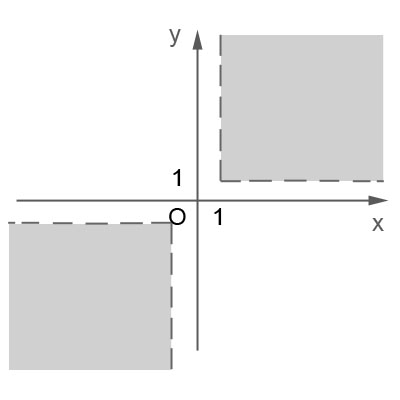
\includegraphics[width=0.4\textwidth]{WA021A.jpg}
  \end{center}
\end{figure}
% -  -  -  -  -  -  -  -  -  -  -  -  -  -  -  -  -  -  -  -  -  -  -  -  -  -  -  -  -  -  
% PART B
\item The function is not defined when the denominator is zero, so we require that $yx^2+xy^2\ne0$, or $xy(x+y)\ne0$. This implies that the function is not defined along the lines $x=0$, $y=0$, and $y=-x$. Moreover, the numerator has a square root. The argument must be non-negative, and so we also have the restriction that $y\ge-1$. The domain can therefore be expressed as $D=\{(x,y)| y\ge -1, x\ne0, y\ne0, y\ne-x\}$. The numerator can take on any non-negative value, and the denominator can take on any value, so the function $f$ can take on any value, so the range is $\mathbb{R}$.
\begin{figure}[!htbp]
  \begin{center}
    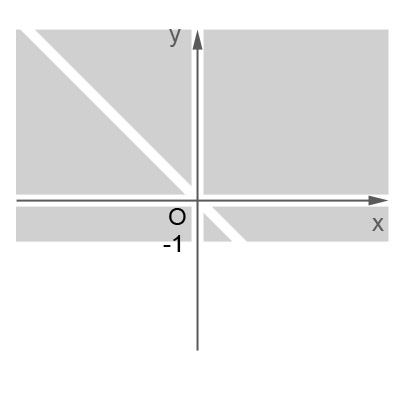
\includegraphics[width=0.4\textwidth]{WA021B.jpg}
  \end{center}
\end{figure}
% -  -  -  -  -  -  -  -  -  -  -  -  -  -  -  -  -  -  -  -  -  -  -  -  -  -  -  -  -  -  
% PART C
\item The function is not defined when the denominator is zero, so we require that $x^2+y^2\ne1$. The domain can therefore be expressed as $D=\{(x,y)| x^2+y^2 \ne 1 \}$. The numerator can take on any value, so the function $f$ can take on any value, so the range is $\mathbb{R}$.
\begin{figure}[!htbp]
  \begin{center}
    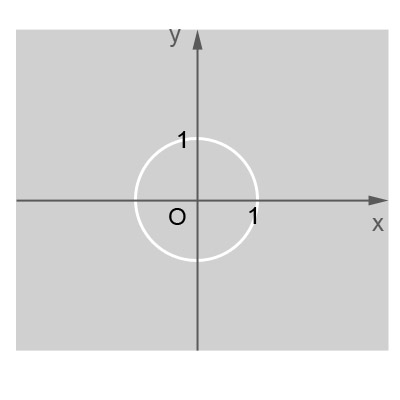
\includegraphics[width=0.4\textwidth]{WA021C.jpg}
  \end{center}
\end{figure}
% -  -  -  -  -  -  -  -  -  -  -  -  -  -  -  -  -  -  -  -  -  -  -  -  -  -  -  -  -  -  
% PART D
\newpage
\item For the domain, we require that 
\begin{align*}
x+2y &> 0  \text{, or } y > - x/2.
\end{align*}
The domain can therefore be expressed as $D=\{(x,y)|y > - x/2\}$. The function $f$ can take on any value, so the range is $\mathbb{R}$.
\begin{figure}[!htbp]
  \begin{center}
    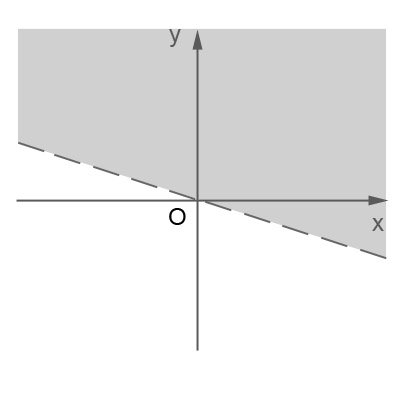
\includegraphics[width=0.4\textwidth]{WA021D.jpg}
  \end{center}
\end{figure}
% -  -  -  -  -  -  -  -  -  -  -  -  -  -  -  -  -  -  -  -  -  -  -  -  -  -  -  -  -  -  
\end{enumerate}

% ~~~~~~~~~~~~~~~~~~~~~~~~~~~~~~~~~~~~~~~~~~~~~~~~~~~~~~~~~
\item
% LIMIT SOLUTIONS
% -  -  -  -  -  -  -  -  -  -  -  -  -  -  -  -  -  -  -  -  -  -  -  -  -  -  -  -  -  -  
\begin{enumerate}
\item We can simply evaluate the limit to obtain
\begin{align*}
\lim_{(r,s)\rightarrow(0,2\pi) } \frac{3r^2+rs^3-3\sin (s/4)}{r^2}
&= \lim_{(r,s)\rightarrow(0,2\pi) }3+\frac{s^3}{r}-3r^2\sin (s/4)
\end{align*}
Because of the $s^3/r$ term, this limit tends to infinity, and therefore does not exist.
% -  -  -  -  -  -  -  -  -  -  -  -  -  -  -  -  -  -  -  -  -  -  -  -  -  -  -  -  -  -  
\item Let $f(x,y) = (x-y)/(x+y)$. Along the $x$-axis, $f=f(x,0)$, so 
\begin{align*}
f(x,0) = \frac{x}{x} = 1, \quad x\ne 0.
\end{align*}
A similar calculation shows that along the $y$-axis, $f$ = -1, if $y\ne0$. If we approach the point $(0,0)$ along the $x$-axis and the $y$-axis, we find that 
\begin{align*}
\text{along the $x$-axis, } & f = f(x,0),\text{ and } f \rightarrow +1 \\
\text{along the $y$-axis, } & f = f(0,y),\text{ and } f \rightarrow -1 
\end{align*}
These limits are not equal, and so the limit does not exist. 
% -  -  -  -  -  -  -  -  -  -  -  -  -  -  -  -  -  -  -  -  -  -  -  -  -  -  -  -  -  -  
\item We can simply evaluate the limit to obtain 
\begin{align*}
  \lim_{(x,y,z)\rightarrow(1,1,1)} \big|3x - 2y - z \big| = 3 -2 -1 = 0
\end{align*}
% -  -  -  -  -  -  -  -  -  -  -  -  -  -  -  -  -  -  -  -  -  -  -  -  -  -  -  -  -  -  
\item  Let $f(x,y,z) = (x^2-y^2-z^2)/(x^2+y^2+z^2)$. Then, along the $x$-axis, $f=(x,0,0)$. As long as $x$ is not zero, $f$ is equal to 1. However, along the $y$-axis, $f=f(0,y,0)$. Provided that $y$ is not zero, $f$ is equal to -1. Therefore,
\begin{align*}
\text{along the $x$-axis, } & f \rightarrow +1 \\
\text{along the $y$-axis, } & f \rightarrow -1 
\end{align*}
These limits are not equal, and so the limit does not exist. 
% -  -  -  -  -  -  -  -  -  -  -  -  -  -  -  -  -  -  -  -  -  -  -  -  -  -  -  -  -  -  
\item  We can evaluate this limit by rationalizing the numerator.
\begin{align*}
  \lim_{(x,y)\rightarrow(1,0) } \frac{\sqrt{2x+y}-\sqrt{2x-y}}{2y} &= 
  \lim_{(x,y)\rightarrow(1,0) } \frac{\sqrt{2x+y}-\sqrt{2x-y}}{2y} \Bigg(\frac{\sqrt{2x+y}+\sqrt{2x-y}}{\sqrt{2x+y}+\sqrt{2x-y}} \Bigg) \\
  &=\lim_{(x,y)\rightarrow(1,0) } \frac{(2x+y)-(2x-y)}{2y \Big(\sqrt{2x+y}+\sqrt{2x-y} \Big)}  \\
  &=\lim_{(x,y)\rightarrow(1,0) } \frac{2y}{2y \Big(\sqrt{2x+y}+\sqrt{2x-y} \Big)}  \\
  &=\lim_{(x,y)\rightarrow(1,0) } \frac{1}{\sqrt{2x+y}+\sqrt{2x-y} }  \\
  &= \frac{1}{2\sqrt{2} }\\
  &= \frac{\sqrt{2}}{2}
\end{align*}
% -  -  -  -  -  -  -  -  -  -  -  -  -  -  -  -  -  -  -  -  -  -  -  -  -  -  -  -  -  -  
\end{enumerate}
% ~~~~~~~~~~~~~~~~~~~~~~~~~~~~~~~~~~~~~~~~~~~~~~~~~~~~~~~~~
\item
% CONTINUITY 
The given function is defined everywhere. Now, for it to be continuous at any point $(x_0,y_0,z_0)$, we require that 
\begin{align*} 
   \lim_{(x,y,z)\rightarrow(x_0,y_0,z_0) } g(x,y,z) = g(x_0,y_0,z_0)
 \end{align*}
If we evaluate the limit as $g$ approaches $(0,0,1)$, we have
\begin{align*}
\lim_{(x,y,z)\rightarrow(0,0,1) } f(x,y,z) 
&= \lim_{(x,y,z)\rightarrow(0,0,1) } x+y+2z \\
&= 0+0+2(1) \\
&= 2
\end{align*}
However, at $(0,0,1)$, $g = 2$. So the given function is not continuous at the point $(0,0,1)$. Elsewhere, the function is a polynomial in three variables, and so will be continuous everywhere except at the point $(0,0,1)$. 
% ~~~~~~~~~~~~~~~~~~~~~~~~~~~~~~~~~~~~~~~~~~~~~~~~~~~~~~~~~
\item The lines $y=m(x-1)$ all pass through the limit point, $(1,0)$, where $m$ is any real number. Approaching the limit point along these lines, our limit becomes
\begin{align*} 
   \lim_{(x,y)\rightarrow(1,0) } \frac{x(x-1)^3 + y^2}{4(x-1)^2+9y^3} 
   &= \lim_{(x,y)\rightarrow(1,0) } \frac{x(x-1)^3 + m^2(x-1)^2}{4(x-1)^2+9m^3(x-1)^3} \\
   &= \lim_{(x,y)\rightarrow(1,0) } \frac{x(x-1) + m^2}{4+9(x-1)} \\
   &= \frac{m^2}{4}
 \end{align*}
 The result depends on $m$, which is an arbitrary value. Therefore, the limit does not exist. 
% ~~~~~~~~~~~~~~~~~~~~~~~~~~~~~~~~~~~~~~~~~~~~~~~~~~~~~~~~~

\item
\begin{enumerate}
\item To plot the level curves, we set $z = c$, and solve for $y$: 
\begin{align*} 
  c &= \frac{\ln y}{x^2} \\
  cx^2&= \ln y \\
  y &= e^{cx^2}
\end{align*}
\begin{figure}[!htbp]
  \begin{center}
    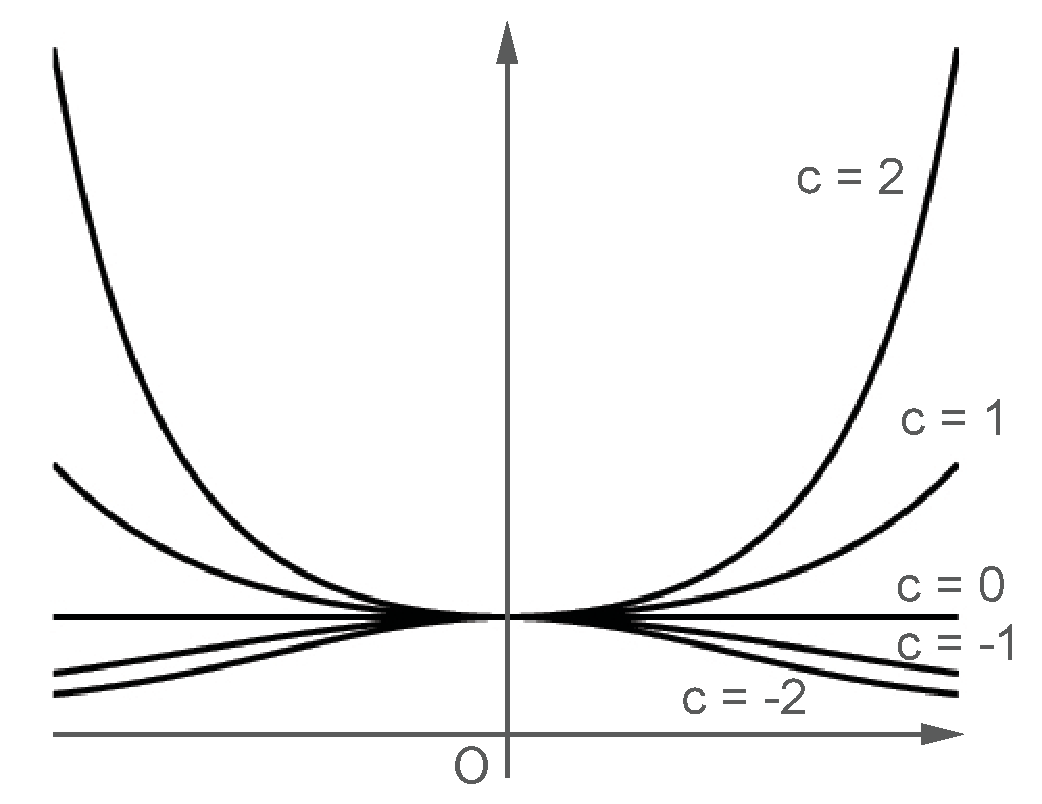
\includegraphics[width=0.4\textwidth]{LevelCurvesA.pdf}
  \end{center}
\end{figure}
% -  -  -  -  -  -  -  -  -  -  -  -  -  -  -  -  -  -  -  -  -  -  -  -  -  -  -  -  -  -  
\item To plot the level curves, we set $z = c$, and solve for $y$: 
\begin{align*} 
  c &= \frac{x^2}{x^2+y^2} \\
  cy^2 &= (1-c)x^2
\end{align*}
If $c=0$, then we obtain the level curve $x = 0$. If $c \ne0$, then
\begin{align*} 
  y &= \pm \sqrt{\frac{1-c}{c}}x, \quad c \ne0
\end{align*}
For $c=2$, $y$ is undefined, so the level curves do not exist. The level curves for the other values of $c$ are shown in the graph below and are as follows:
\begin{align*} 
  \text{if } c&=0, \quad x = 0 \text{ (the vertical line that lies on the } y \text{-axis})\\
  \text{if } c&=1/4, y = \pm \sqrt{3}x\\
  \text{if } c&=1/2, y = \pm x\\  
  \text{if } c&=1, \quad y = 0    
\end{align*}

\begin{figure}[!htbp]
  \begin{center}
    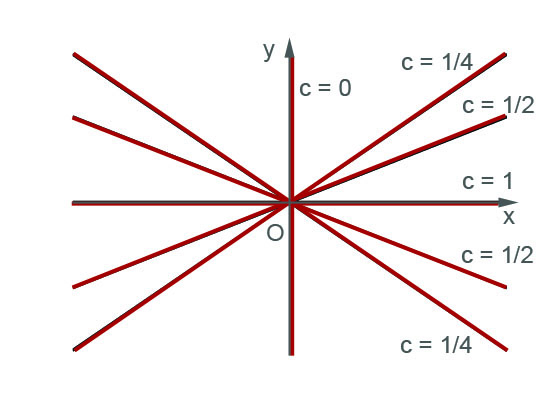
\includegraphics[width=0.4\textwidth]{LevelCurvesB.jpg}
  \end{center}
\end{figure}

\end{enumerate}
% ~~~~~~~~~~~~~~~~~~~~~~~~~~~~~~~~~~~~~~~~~~~~~~~~~~~~~~~~~
\item
\begin{enumerate}
\item The set of straight lines that pass through $(2,1)$ are given by $y = c(x-2) + 1$. Rearranging yields the equation 
\begin{align*}
c = \frac{y-1}{x-2}
\end{align*}
The desired function is 
\begin{align*}
f(x,y) = \frac{y-1}{x-2}
\end{align*}
\item The set of circles with radius $e^c$ are given by $x^2 + y^2 = e^c$. Applying the natural logarithm to both sides of the equation yields 
\begin{align*}
\ln(x^2+y^2) = c
\end{align*}
The desired function is 
\begin{align*}
f(x,y) =\ln(x^2+y^2)
\end{align*}\end{enumerate}
% ~~~~~~~~~~~~~~~~~~~~~~~~~~~~~~~~~~~~~~~~~~~~~~~~~~~~~~~~~
% PROVIDE EXAMPLE, LIMIT
\item 
\begin{enumerate}
\item
Suppose we let 
\begin{align*}
f(x,y) = \frac{y}{(x-1)^2}
\end{align*}
Then, along any parabola $y = m(x-1)^2$ the limit becomes
\begin{align*}
\lim_{(x,y)\rightarrow(1,0) } \frac{y}{(x-1)^2} = \lim_{(x,y)\rightarrow(1,0) } \frac{m(x-1)^2}{(x-1)^2} = m
\end{align*}
The function we chose therefore meets the specified criteria.
\item
The limit cannot exist because the limit depends on $m$, which is an arbitrary real number.
\end{enumerate}
% ~~~~~~~~~~~~~~~~~~~~~~~~~~~~~~~~~~~~~~~~~~~~~~~~~~~~~~~~~
% TEMPERATURE DISTRIBUTION
\item 
\BEN
\item The temperature can be written as 
\begin{align*}T(x,y) = \frac{k}{\sqrt{x^2 + y^2}},\end{align*} 
where $k$ is an unknown constant of proportionality.
\item The level curves are solution sets of the equation $T(x,y)=c$, for $c\in\R$. Therefore,
\begin{align*}
  T(x,y) = c &= \frac{k}{\sqrt{x^2 + y^2}} \\
  c^2 &= \frac{k^2}{x^2 + y^2} \\
  x^2 + y^2 &= \frac{k^2}{c^2}
\end{align*} 
The level curves are concentric circles with radius $k/c$. 
\item At the point (2,1), the temperature is known, which allows us to solve for $k$. 
\begin{align*}
  T(2,1) = 10 &= \frac{k}{\sqrt{2^2 + 1^2}}\\
  k& = 10\sqrt{5}
\end{align*} 
At (1,3), the temperature is
\begin{align*}
  T(1,3) &= \frac{10\sqrt{5}}{\sqrt{1^2 + 3^2}}\\
  & = 10\sqrt{\frac{5}{4}}
\end{align*} 
\EEN
% ~~~~~~~~~~~~~~~~~~~~~~~~~~~~~~~~~~~~~~~~~~~~~~~~~~~~~~~~~
% ELECTRIC POTENTIAL DISTRIBUTION
\item The level curves are solution sets of the equation $V(x,y) = K$, for constant $K\in\R$.
\begin{align*}
V(x,y) = K &= \frac{c}{\sqrt{r^2 - x^2 -y^2}} \\
r^2-x^2-y^2 &= \frac{c^2}{K^2} \\
x^2+y^2 &= r^2 -  \frac{c^2}{K^2}
\end{align*}
The left-hand side must be positive, so we must have that 
\begin{align*}
r^2 &>  \frac{c^2}{K^2}\\
K^2 &> c^2/r^2\\
 |K| &<  |c|/|r|
\end{align*}
But $c, K$, and $r$ are all positive constants, so this simplifies to $K<\frac{c}{r}$. The level curves are concentric circles, centered at the origin, with radius $r^2 -  \frac{c^2}{K^2}$, for $K<\frac{c}{r}$.
% ~~~~~~~~~~~~~~~~~~~~~~~~~~~~~~~~~~~~~~~~~~~~~~~~~~~~~~~~~
% LIMIT PROOF
\item 
If we approach the limit point along the $x$-axis, then $y=0$ and we obtain
\begin{align*}
  \lim_{(x,y)\rightarrow(0,0) } \frac{x(0)^2}{x^2+(0)^2} = 0
\end{align*}
We obtain the same result if we approach the origin along the $y$-axis, or along any line $y=mx$. It would seem that the limiting value could exist and could be equal to 0. To show that this is the case, we must show that for any $\epsilon > 0$, there exists a $\delta > 0$ such that   
\begin{align*}
 \Big|  \frac{xy^2}{x^2+y^2} - 0 \Big| < \epsilon \text{  whenever  } 0 < \sqrt{(x-0)^2 + (y-0)^2} < \delta ,
\end{align*}
or simply
\begin{align*}
 \Big|  \frac{xy^2}{x^2+y^2} \Big| < \epsilon \text{  whenever  } 0 < \sqrt{x^2 + y^2} < \delta .
\end{align*}
Now, $\big| x^2 + y^2\big| = x^2 + y^2$, and $|y^2| = y^2$, so
\begin{align*}
 \Big|  \frac{xy^2}{x^2+y^2} \Big| &=  \frac{ \big|xy^2 \big|}{ \big|x^2+y^2 \big|}  =   \frac{ \big|x\big|y^2 }{ x^2+y^2 }
\end{align*}
Also, $|x| \le \sqrt{x^2+y^2}$, and $y^2 \le x^2+y^2$, so
\begin{align*}
 \Big|  \frac{xy^2}{x^2+y^2} \Big| 
 &=  \frac{ \big|x\big|y^2 }{ x^2+y^2 }\\
 &\le \frac{ \ \sqrt{x^2+y^2} ( x^2+y^2 ) }{ x^2+y^2 }\\
 &= \sqrt{x^2+y^2}
\end{align*}
So if $\delta = \epsilon$, then 
\begin{align*}
 \Big|  \frac{xy^2}{x^2+y^2} \Big| < \epsilon \text{  whenever  } 0 < \sqrt{x^2 + y^2} < \delta .
\end{align*}
% ~~~~~~~~~~~~~~~~~~~~~~~~~~~~~~~~~~~~~~~~~~~~~~~~~~~~~~~~~

\end{enumerate}

\end{document}
